% !TEX program = lualatex
\documentclass[11pt]{article}

% -------- LuaLaTeX : polices et langue --------
\usepackage{fontspec}
\setmainfont{Latin Modern Roman}
\setsansfont{Tex Gyre Heros}
%\renewcommand{\familydefault}{\sfdefault} % force le sans serif par défaut
\usepackage{polyglossia}
\setdefaultlanguage{french}

% -------- Mise en page --------
\usepackage[a4paper,margin=1cm]{geometry}
\usepackage{multicol}
\usepackage{fancyhdr}
\pagestyle{empty}
\usepackage[most]{tcolorbox}

% -------- Mathématiques --------
\usepackage{amsmath,amssymb,mathtools}
% \usepackage{siunitx}
% \sisetup{locale=FR}

\usepackage{enumitem}
\setlist[itemize]{left=0pt}
\setlist[enumerate]{left=0pt, label=\textbf{\arabic*}.}

\usepackage{ProfCollege}
\usepackage{ProfMaquette}

%\usepackage{tabularray}
\usepackage{tabularx}

% -------- Divers --------
\newcommand{\ligne}{{\color{gray!60}\hrulefill}}

\setlength{\parindent}{0pt}

\begin{document}

\begin{Maquette}[DM]{
        Numero = 1, Code={}, Date = jeudi 16 octobre 2025, Niveau = Quatrième
    }

    \begin{exercice}
        \brm{5}
        Sur le quadrillage ci-dessous,
        \begin{enumerate}
            \item trace l’image de la lettre F par la symétrie d’axe (AB)
            \item trace ensuite l’image du motif formé par les deux lettres F par la translation qui transforme I en J, c’est-à-dire de vecteur $\overrightarrow{\textrm{IJ}}$
        \end{enumerate}
        \begin{center}
            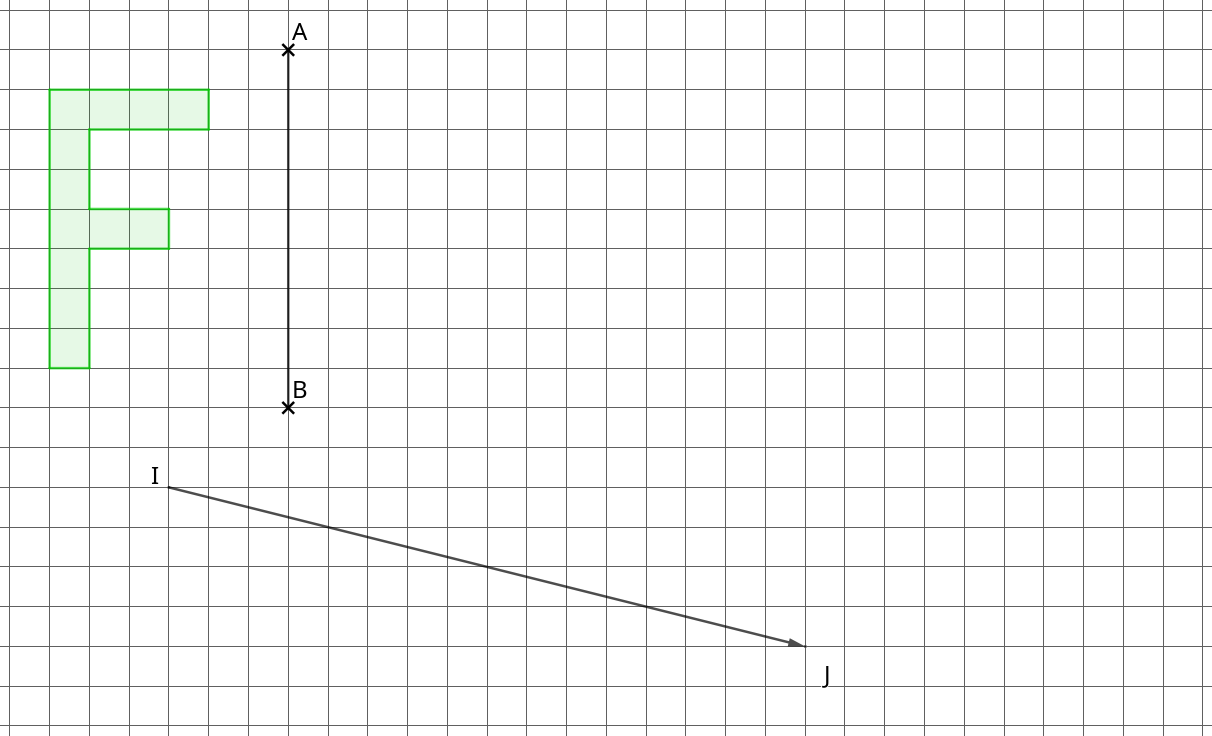
\includegraphics[width=\linewidth]{Images/Exercice1.png}
        \end{center}
    \end{exercice}
    
    \begin{exercice}
        \brm{5}
        Réduis chaque expression littérale. (Si elle ne peut pas être réduite, recopie-la.)
        \setlength{\columnsep}{1cm}
        \begin{multicols}{3}
            \begin{enumerate}[itemsep=1em]
                \item $A = 5 x \times 3 =$ \ligne
                \item $B = 5 + 3x = $ \ligne
                \item $C = 3 \times 5x =$ \ligne
                \item $D = 5x + 3x =$ \ligne
                \item $E = 5x \times 3x =$ \ligne
                \item $F = 5x - 3x =$ \ligne
                \item $G = 5x + 3 =$ \ligne 
                \item $H = 5x^2 + 3x = $ \ligne
                \item $I = 5x^2 + 3x^2 = $ \ligne
                \item $J = 5 + 3 \times x = $ \ligne
            \end{enumerate}
        \end{multicols}
    \end{exercice}

\end{Maquette}


\end{document}